\documentclass{article}
\usepackage[utf8]{inputenc}
\usepackage[left=1in,right=1in,top=1in,bottom=1in]{geometry}
\usepackage{crop,graphicx,array,color,flushend,stfloats,amsthm,chngpage,times,fancyhdr,lipsum,lastpage}

%%%%%%%%%%%%   Extra libraries & settings %%%%%%%%%%%%%
\setlength{\parskip}{0.25em}

%%%%%%%%%%%%   Header and Footer  %%%%%%%%%%%%%
\pagestyle{fancy}

\fancypagestyle{plain}{%
  \renewcommand{\headrulewidth}{0pt}%
  \fancyhf{}%
  \fancyfoot[R]{Page \bf\thepage\ \rm of \bf\pageref{LastPage}}%
}


%%%% Customise Titles and Headers: %%%%
\title{Don't forget adding title}
\author{Chinchuthakun Worameth (18B00033)}
\date{\today}

\fancyhf{}
\fancyhead[L]{Chinchuthakun Worameth}
\fancyhead[R]{18B00033}
\fancyfoot[R]{Page \bf\thepage\ \rm of \bf\pageref{LastPage}}


\AtBeginDocument{
%%%%%%%%%%%% Make Title and Format Lines %%%%%%%%%%%%
\maketitle											%
\vspace{-120px}										%
\noindent\rule{\linewidth}{1pt} \par				%
\vspace{100px}										%
\vspace{-20px}										%
\noindent\rule{\linewidth}{1pt} \par				%
\vspace{10px}										%
% %%%%%%%%%%%%%%%%%%% Content %%%%%%%%%%%%%%%%%%%%	
}

\AtEndDocument{
\bibliographystyle{IEEEtran}
\nocite{*}
\bibliography{citation}
}
% math stuff
\usepackage{amsmath}                % to use DeclareMathOperator
\usepackage{amssymb}
\usepackage{mathrsfs}
\usepackage{mathtools}
\usepackage{xargs}                  % for more than one optional arguments when define new commands
\usepackage{physics}                % vectors
\usepackage{mdframed}               % frames for definition, theorem, etc.
\usepackage[ruled]{algorithm2e}     % for algorithms
\usepackage{ifthen}                % for \ifthenelse
\usepackage{upgreek}

% figures and tables
\usepackage{titlesec}
\usepackage{caption}
\usepackage{subcaption}
\usepackage{multirow}
\usepackage{relsize}

% formatting some important single letters
\renewcommand{\epsilon}{\varepsilon}
\renewcommand{\phi}{\varphi}
\renewcommand{\upepsilon}{\upvarepsilon}
\renewcommand{\upphi}{\upvarphi}

% new operators
\DeclareMathOperator*{\argmin}{arg\,min}                % argmin
\DeclareMathOperator*{\argmax}{arg\,max}                % argmax
\DeclarePairedDelimiter\ceil{\lceil}{\rceil}            % ceiling function
\DeclarePairedDelimiter\floor{\lfloor}{\rfloor}         % floor function
\DeclarePairedDelimiter{\parens}{\lparen}{\rparen}      % parenthesis (use \parens* for automatically adjusting version)
\DeclarePairedDelimiter{\bracket}{[}{]}
\DeclarePairedDelimiter{\cbracket}{\{}{\}}
\DeclarePairedDelimiter{\ang}{\langle}{\rangle}
% \DeclarePairedDelimiter{\fourier}{\mathscr{F}\{}{\}}
% \DeclarePairedDelimiter{\invfourier}{\mathscr{F}^{-1}\{}{\}}

\newcommand{\fourier}[1]{\mathscr{F}\cbracket*{#1}}
\newcommand{\invfourier}[1]{\mathscr{F}^{-1}\cbracket*{#1}}
\newcommand {\dx}{\,dx}
\newcommand {\dy}{\,dy}
\newcommand {\dz}{\,dz}
\newcommand {\dt}{\,dt}
\newcommand {\du}{\,du}
\newcommand {\dtheta}{\,d\theta}
\newcommand {\domega}{\,d\omega}



\newcommand{\bigo}[1]{\ensuremath{\mathcal{O}\parens*{#1}}}
% new commands
\newcommand{\st}{such that }
\newcommand{\w}{where }
\newcommand{\del}{\nabla}
\newcommand{\larrow}{\leftarrow}
\newcommand{\rarrow}{\rightarrow}
\newcommand{\tbf}{\textbf}
\newcommand{\tit}{\textit}
\newcommand{\col}{\operatorname{col}}
\newcommand{\mat}[1]{\begin{matrix} #1 \end{matrix}}
% \newcommand{\vect}[1]{\boldsymbol{\mathbf{#1}}}
\newcommand{\vf}[1]{\boldsymbol{\mathbf{#1}}}
\newcommandx*{\seq}[2][1,2]{\ensuremath{#1, \ldots, #2}}
\newcommandx*{\ssum}[3][1,2,3]{\ensuremath{\sum_{#1 = #2}^{#3}}}
\newcommandx*{\sint}[2][1,2]{\ensuremath{\int_{#1}^{#2}}}
% \newcommandx*{\func}[4][1,2,3,4]{\ensuremath{#1^{\parens{#2}}_{#3}\parens{#4}}}
% \newcommandx*{\val}[3][1,2,3]{\ensuremath{#1^{\parens{#2}}_{#3}}}

% \newcommandx*{\func}[4][1=f,2=x,3,4, usedefault]{
%     \ifthenelse{\equal{#3}{}}{\ensuremath{#1_{#4}\parens{\vf{#2}}}}{\ensuremath{#1^{\parens{#3}}_{#4}\parens{\vf{#2}}}}
% }
\newcommandx*{\func}[3][1=f,2,3, usedefault]{
    \ifthenelse{\equal{#2}{}}{\ensuremath{#1_{#3}}}{\ensuremath{#1^{\parens{#2}}_{#3}}}
}
\newcommandx*{\val}[3][1,2,3, usedefault]{
    \ifthenelse{\equal{#2}{}}{\ensuremath{\vf{#1}_{#3}}}{\ensuremath{\vf{#1}^{\parens{#2}}_{#3}}}
}

\newcommandx*{\Real}[1][1, usedefault]{\ensuremath{\mathbb{R}^{#1}}}                % set of real number
\newcommandx*{\Int}[1][1, usedefault]{\ensuremath{\mathbb{Z}^{#1}}}                 % set of integer
\newcommandx*{\Natural}[1][1, usedefault]{\ensuremath{\mathbb{N}^{#1}}}             % set of natural number
\newcommandx*{\normal}[2][1=0, 2=1, usedefault=!]{\ensuremath{\mathcal{N}(#1,#2)}}  % Gaussian distribution

% define frame environment
% \newmdtheoremenv{definition}{Definition}
% \newmdtheoremenv{proposition}{Proposition}
% \newmdtheoremenv{corollary}{Corollary}
% \newmdtheoremenv{lemma}{Lemma}
% \newmdtheoremenv{theorem}{Theorem}
% \newmdtheoremenv{remark}{Remark}

% define keywords for algorithm
\SetKwInOut{Input}{Input}
\SetKwInOut{Output}{Output}
\SetKwInOut{Parameter}{Parameter}

% \begin{theorem}{text}{label}
% refer as \ref{tha:label}
\usepackage{tcolorbox}
\tcbuselibrary{theorems,breakable} %% を読み込む
\definecolor{burgundy}{rgb}{0.5, 0.0, 0.13}
\newtcbtheorem[number within=section]{theorem}{Theorem}%
{colframe=burgundy,colback=burgundy!2!white,
rightrule=0pt,leftrule=0pt,bottomrule=2pt,
colbacktitle=burgundy,theorem style=standard,breakable,arc=0pt}{theo}

\definecolor{oxfordblue}{rgb}{0.0, 0.13, 0.28}
\newtcbtheorem[number within=section]{definition}{Definition}%
{colframe=oxfordblue,colback=oxfordblue!2!white,
rightrule=0pt,leftrule=0pt,bottomrule=2pt,
colbacktitle=oxfordblue,theorem style=standard,breakable,arc=0pt}{def}

\definecolor{cadmiumorange}{rgb}{0.93, 0.53, 0.18}
\newtcbtheorem[number within=section]{remark}{Remark}%
{colframe=cadmiumorange,colback=cadmiumorange!2!white,
rightrule=0pt,leftrule=0pt,bottomrule=2pt,
colbacktitle=cadmiumorange,theorem style=standard,breakable,arc=0pt}{rem}

% equation numbering
\numberwithin{equation}{section}

%%%%%%%%%%%%%%%%%%%%%%%%%%%
\usepackage{listings}
\usepackage{xcolor}

\definecolor{codegreen}{rgb}{0,0.6,0}
\definecolor{codegray}{rgb}{0.5,0.5,0.5}
\definecolor{codepurple}{rgb}{0.58,0,0.82}
\definecolor{backcolour}{rgb}{0.95,0.95,0.92}

\lstdefinestyle{mystyle}{
    backgroundcolor=\color{backcolour},   
    commentstyle=\color{codegreen},
    keywordstyle=\color{magenta},
    numberstyle=\tiny\color{codegray},
    stringstyle=\color{codepurple},
    basicstyle=\ttfamily\footnotesize,
    breakatwhitespace=false,         
    breaklines=true,                 
    captionpos=b,                    
    keepspaces=true,                 
    numbers=left,                    
    numbersep=5pt,                  
    showspaces=false,                
    showstringspaces=false,
    showtabs=false,                  
    tabsize=2
}

\lstset{style=mystyle}

\makeatletter
\renewcommand*\env@matrix[1][\arraystretch]{%
  \edef\arraystretch{#1}%
  \hskip -\arraycolsep
  \let\@ifnextchar\new@ifnextchar
  \array{*\c@MaxMatrixCols c}}
\makeatother
\usepackage{subfiles}
\usepackage{subcaption}
\usepackage{tikz}
\title{Computer Graphics Assignment \#4}
\begin{document}
\section{Question}
There are three cubes, which are the sun, the earth and the moon, in the window of the sample program. However those star motions are different from real motions.
\begin{enumerate}
    \item Change the code to animate the stars as real as possible in the sun coordinate system. It means that the sun is fixed, the revolution (round the sun) and rotation of the earth, and the revolution (round the earth) and rotaton of the moon.
    \item Describe the equations for each stars with a time $t$, where $t = 365$ is corresponding to one year. Capture the animation window and put on your report.
\end{enumerate}
In both answers, include efficient images or graphs to help the understanding of the explanations.

\section{Answer}

Suppose that star motions, e.g. earth around sun and moon around earth, are circular on the 2D Cartesian coordinate system centered at the sun, as illustrated in Figure \ref{cg4-diagram}. We further assume the following:
\begin{enumerate}
    \item Ratio of distance between stars $d_1:d_2 = 6:3$.
    \item Ratio of dimension of stars $r_1:r_2:r_3 = 1:0.3:0.06$.
    \item Period of the earth's circular motion around the sun is 365 days.
    \item Period of the moon's circular motion around the earth is 27.3 days. Since $365 / 27.3$ is not an integer, the position of the moon at the beginning of each month is slightly shifted from the previous one.
    \item Ignore earth's rotation and moon's rotation.
\end{enumerate}
\subfile{./figures/assignment4/cg4-diagram}
Based on these assumptions, we can describe the position of each star at time $t \in \Real$ as Equation \eqref{eq-sun}, \eqref{eq-earth} and \eqref{eq-moon}.

\begin{subequations}
    \begin{gather}
    \begin{bmatrix}[1.25]
    x_S(t) \\
    y_S(t) \\
    z_S(t) \\
    1
    \end{bmatrix} = 
    \begin{bmatrix}[1.25]
    1 & 0 & 0 & 0 \\
    0 & 1 & 0 & 0 \\
    0 & 0 & 1 & -18 \\
    0 & 0 & 0 & 1
    \end{bmatrix} 
    \begin{bmatrix}[1.25]
    x_O(t) \\
    y_O(t) \\
    z_O(t) \\
    1
    \end{bmatrix}
    \label{eq-sun}
    \\
    \begin{bmatrix}[1.25]
    x_E(t) \\
    y_E(t) \\
    z_E(t) \\
    1
    \end{bmatrix} = 
    \begin{bmatrix}[1.25]
    0.3 & 0 & 0 & 0 \\
    0 & 0.3 & 0 & 0 \\
    0 & 0 & 0.3 & 0 \\
    0 & 0 & 0 & 1
    \end{bmatrix} 
    \begin{bmatrix}[1.25]
    1 & 0 & 0 & -d_1\cos\parens*{\text{Mod}\parens*{\frac{360}{365}t,360}} \\
    0 & 1 & 0 & -d_1\sin\parens*{\text{Mod}\parens*{\frac{360}{365}t,360}} \\
    0 & 0 & 1 & 0 \\
    0 & 0 & 0 & 1
    \end{bmatrix} 
    \begin{bmatrix}[1.25]
    x_S(t) \\
    y_S(t) \\
    z_S(t) \\
    1
    \end{bmatrix}
    \label{eq-earth}
    \\
    \begin{bmatrix}[1.25]
    x_M(t) \\
    y_M(t) \\
    z_M(t) \\
    1
    \end{bmatrix} = 
    \begin{bmatrix}[1.25]
    0.2 & 0 & 0 & 0 \\
    0 & 0.2 & 0 & 0 \\
    0 & 0 & 0.2 & 0 \\
    0 & 0 & 0 & 1
    \end{bmatrix} 
    \begin{bmatrix}[1.25]
    1 & 0 & 0 & -d_1\cos\parens*{\text{Mod}\parens*{\frac{360}{27.3}t,360}} \\
    0 & 1 & 0 & -d_1\sin\parens*{\text{Mod}\parens*{\frac{360}{27.3}t,360}} \\
    0 & 0 & 1 & 0 \\
    0 & 0 & 0 & 1
    \end{bmatrix} 
    \begin{bmatrix}[1.25]
    x_E(t) \\
    y_E(t) \\
    z_E(t) \\
    1
    \end{bmatrix}
    \label{eq-moon}
    \end{gather}
\end{subequations}
where subscripts $O, S, E, M$ denote coordinates of original cube, Sun, Earth and Moon, respectively. The function $\text{Mod}(x,y) = \text{rad}\parens*{x - y\floor*{\frac{x}{y}}}$ ensures that arguments of sine and cosine function are always in range $[0,2\pi)$. Note that $x_S(t), y_S(t), z_S(t)$ can be any real number; however, the value in Equation \eqref{eq-sun} is specifically chosen for animation purpose. Figure \ref{cg4-snapshot} shows a snapshot of the animation window displaying the sun-earth-moon system.
\begin{figure}[h]
    \centering
    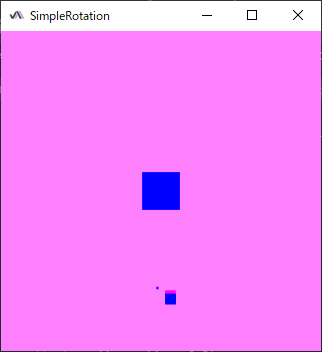
\includegraphics[width=0.4\textwidth]{figures/assignment4/cg4-snapshot.png}
    \caption{A snapshot of the animation window}
    \label{cg4-snapshot}
\end{figure}

\end{document}